% Introduce detector, location, basic info (e.g., chamber count)
% What is the technology
% Anatomy of a chamber
% How are they arranged in the barrel/endcap
% What do they measure
% Coverage
% Performance

Providing coverage in the plus and minus MEs within $0.9<|\eta|<2.4$ are the Cathode Strip Chambers (CSCs), which occupy the four ME stations along with RPCs. CSCs are labeled by ME station $\pm$n, then by ring m, like ``ME$\pm$n/m.'' In ME$\pm$2 to ME$\pm$4, each station consists of two concentric rings of CSCs, while ME$\pm$1 supports three rings of chambers (see Fig.~\ref{fig:CSC}). All rings contain 36 chambers, except for the outer-most rings of stations 2-4 (ME$\pm$2/2, ME$\pm$3/2, and ME$\pm$4/2) which hold only 18 chambers, for a total of 540 CSCs. Within each ring, CSCs are azimuthally overlapping with no gaps, offering full $\phi$ coverage. Each chamber is constructed from seven layers of polycarbonate honeycomb panels, with a gas mixture of 50\% Ar, 40\% CO2, and 10\% CF4 filling the six gaps between the panels. Embedded in a thin FR4 (fire-resistant fiberglass epoxy) surface on each panel are radially-extended cathode strips. Within each gap are azimuthally-running anode wires supplied with 2.9 \SI{3.5}{kV} of voltage. Muons passing through a chamber will locally ionize the gas in each gap, while the high voltage will induce a charge avalanche that drifts toward the cathode strips and an image charge will drift toward the anode wires (see Fig.~\ref{fig:CSCDiagram}). Each chamber provides a spacial resolution of 50 to \SI{140}{\micro\meter} (depending on the chamber) and a timing resolution of \SI{3}{ns}.

\begin{figure}[H]
    \centering
    {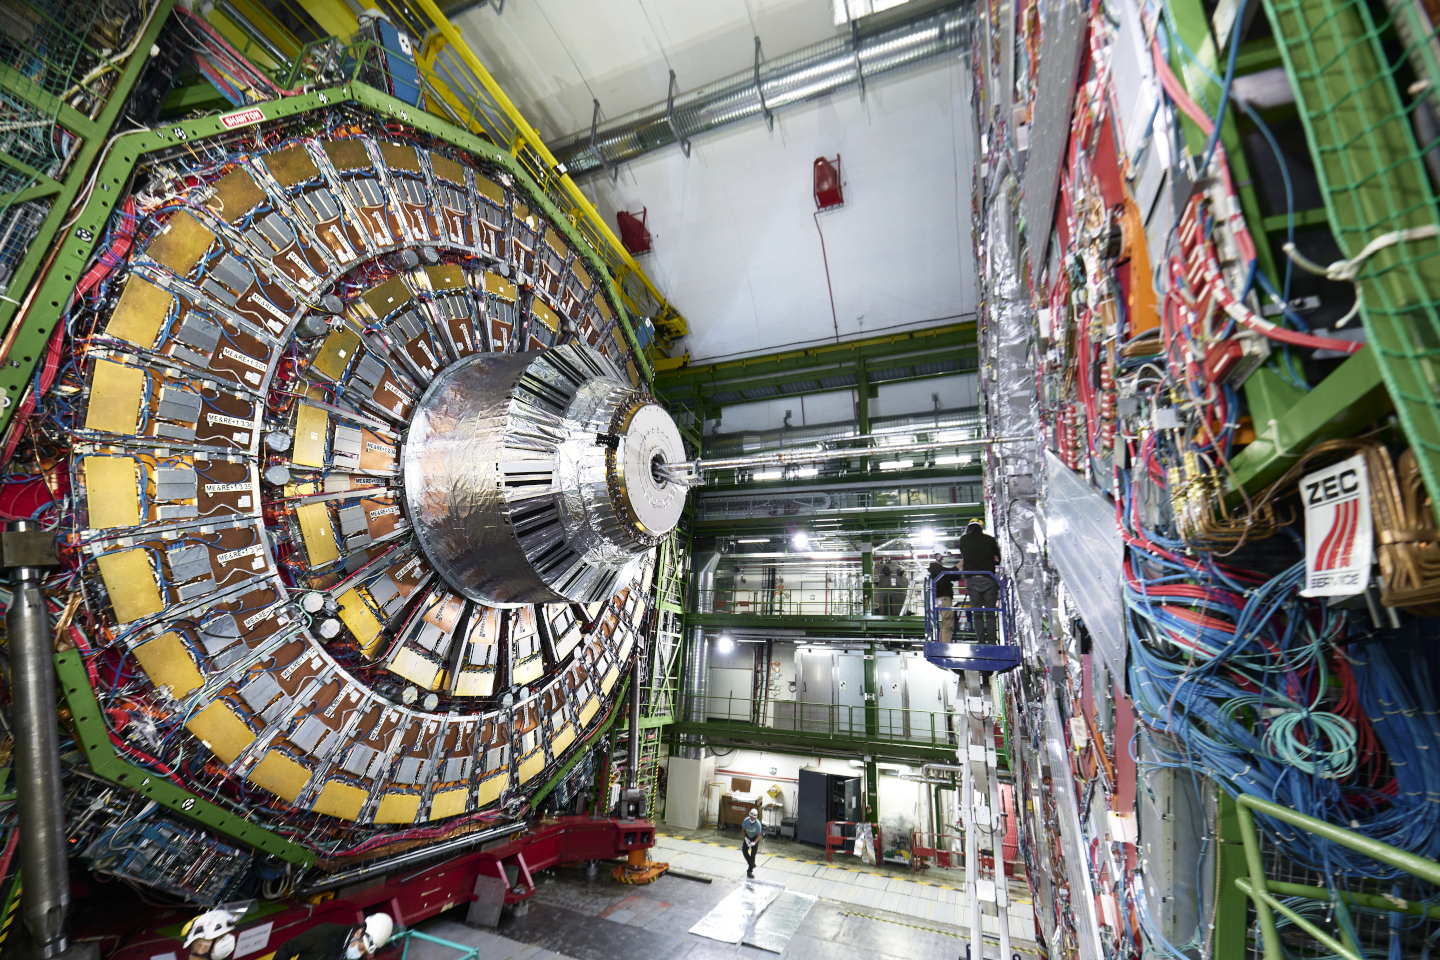
\includegraphics[width=1\textwidth]{Images/CMS/CSC.jpg}}
    \caption{A photograph of CSCs mounted to the first endcap station.}
    \label{fig:CSC}
\end{figure}

\begin{figure}[H]
    \centering
    {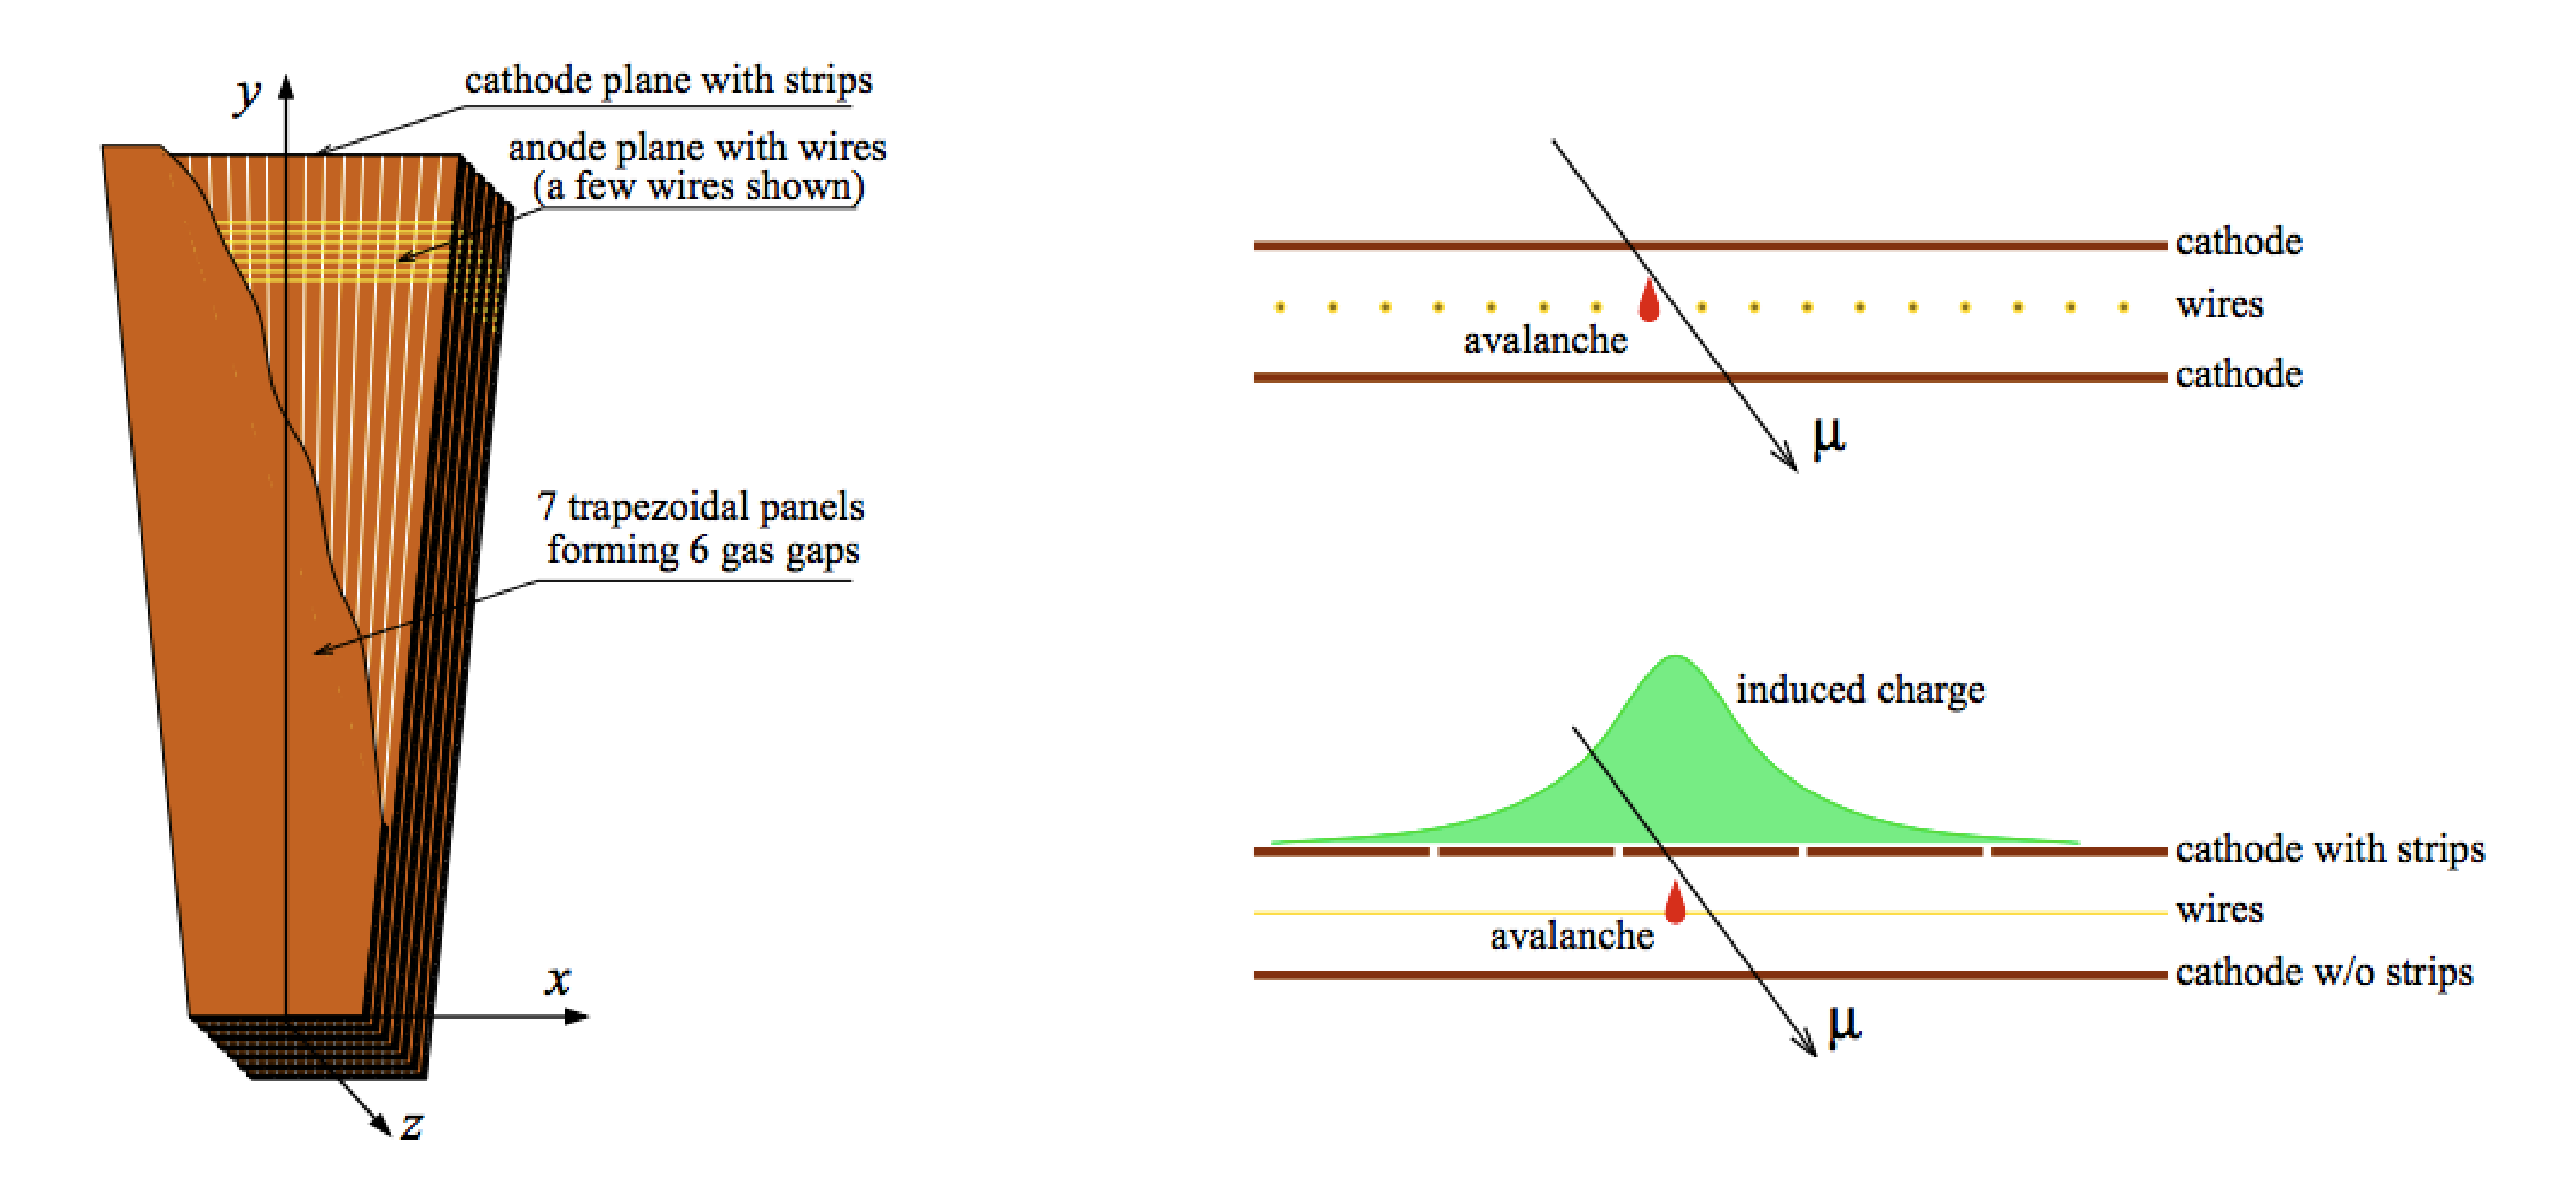
\includegraphics[width=\textwidth]{Images/CMS/CSCDiagram.png}}
    \caption{Left: A schematic of a CSC. Right: A muon passing through a CSC will induce a charge avalanche.}
    \label{fig:CSCDiagram}
\end{figure}